Within the framework of the ESRF Phase II Upgrade Programme, a new state-of-the-art end station for the high-energy beamline ID31 is under development.
Research in many scientific areas such as material and life sciences are increasingly looking for instruments with higher spatial resolution.
The design of the new end station will enable many hard X-ray characterization techniques such as reflectivity, wide angle diffraction and diffraction tomography.
The need of great versatility induces many constrains on the end station such as combining \emph{large stroke} (\(\approx\SI{10}{\milli\metre}\)), \emph{high precision} (\(\approx\SI{10}{\nano\metre}\)) while accepting samples with mass ranging from \(\SI{1}{\kilo\gram}\) to \(\SI{50}{\kilo\gram}\).

Many positioning end stations have been developed with an increasing positioning precision \cite{martinez2016,DucotteMEDSI2016,ogurreck2013nanotomography}.

However, when nanometer precision is needed, thermal expansion and vibrations are becoming the main source of positioning error that cannot be compensated by encoders used for each stage.
Therefore, a direct metrology system is usually needed \cite{DucotteMEDSI2016}.

The aim of this study is to \emph{develop a short stroke Stewart platform that actively stabilize the sample position and compensate for all sources of perturbations and imperfection}.

\begin{tikzfigure}[Schematic of the Tomography Experiment]
\label{fig:exp_full_setup}
\centering
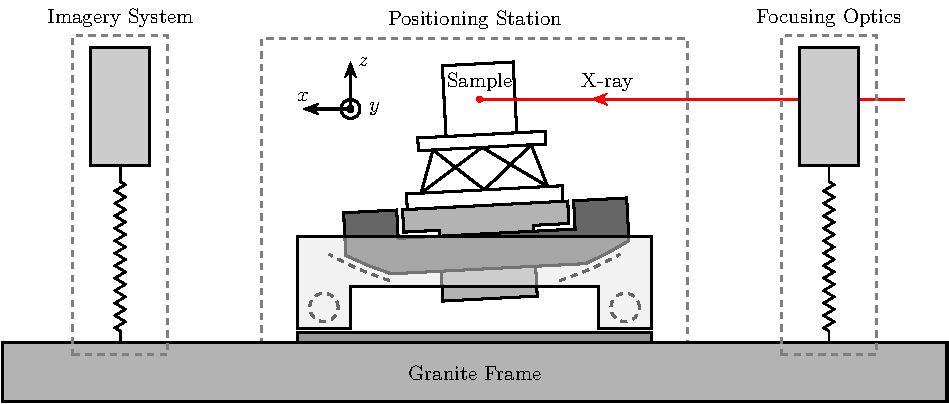
\includegraphics[width=0.95\linewidth]{./figs/exp_full_setup.pdf}


\end{tikzfigure}

%%% Local Variables: ***
%%% mode:latex ***
%%% TeX-master: "2018 - Student Day.tex"  ***
%%% End: ***